\section{Experiments}

This sections contains experiments regarding the architecture of the variational autoencoder (VAE)
and the quality of the latent space. The experiments use the test and validation data of the RGB
imagery as well as the ground truth semantic labeling and the digital surface models as described in
\ref{datasets}.

\subsection{Variational Autoencoder Architecture} \label{architecture_experiments}

The experiments presented in this subsection determine the architecture that is used for the further
experiments regarding the latent space in the next subsection. All the tested VAE architectures have 
latent code of the size $1024$ and are trained with a batch size of $128$, $3000$ images over $50$ epochs.
This is done on the personal computer described in section \ref{hardware}.
The quality of the VAEs is on the one hand measured by the mean absolute error (MAE)
between the reconstruction and the input image.
On the other hand it is judged by the subjective opinion of how realistic the reconstructions look and how well
the semantic contents were recreated. This is the case since the MAE 
cannot capture the visual fidelity of a recreation. For instance if a reconstruction was an image that has the mean
color values of the input as every pixel it is just one color in all of the image and only one value was captured
from the input. However, this result has a lower MAE than an image with the inverted values of the
input. Clearly the inverted image is a much better reconstruction of the input than the unicolored image and therefore
additionally judging the results via a visual inspection is necessary.

The VAE architecture descriptions all cover an encoder up to a one dimensional tensor that is fed into two dense
layers which create the means and standard deviations as explained in section \ref{architecture}. Since these two
dense layers, the resampling and the dimension of the latent code is the same for every architecture the following
specifications of encoders do not include these features for brevity. Additionally the contents of
each figure are only explained in the first architecture because there are the same types of figures for
every test. 
The inputs for every encoder are $128\times 128$ RGB images, i.e. $128\times 128\times 3$ images. The inputs
for every decoder are the latent code vectors of size $1,024$.


\paragraph{Architecture 1}

\begin{center}
    \begin{table}[H]
        \centering
        \begin{tabular}{ | l | c | }
            \multicolumn{2}{c}{Encoder} \\ \hline
            Layer & Output\\ \hline
            Convolution: Kernel $3\times3$, Stride $2\times2$, Filters $8  $    & $64\times 64\times 8  $    \\  
            Convolution: Kernel $3\times3$, Stride $2\times2$, Filters $16 $    & $32\times 32\times 16 $    \\
            Convolution: Kernel $3\times3$, Stride $2\times2$, Filters $32 $    & $16\times 16\times 32 $    \\
            Convolution: Kernel $3\times3$, Stride $2\times2$, Filters $64 $    & $8\times 8\times   64 $    \\
            Convolution: Kernel $3\times3$, Stride $2\times2$, Filters $128$    & $4\times 4\times   128$    \\
            Convolution: Kernel $3\times3$, Stride $2\times2$, Filters $256$    & $2\times 2\times   256$    \\
            Flatten                                                             & $1,024$                    \\
            \hline
        \end{tabular} 
        \caption{The layers of the encoder up to the vector that the two dense layers use to produce 
        the means and standard deviations for the latent code.}
    \end{table}
\end{center}
\vspace{-4em}
\begin{center}
    \begin{table}[H]
        \centering
        \begin{tabular}{ | l | c | }
            \multicolumn{2}{c}{Decoder} \\ \hline
            Layer & Output\\ \hline
            Dense                                                                   & $1,024$                   \\
            Reshape                                                                 & $2\times 2\times    256$  \\
            Deconvolution: Kernel $3\times3$, Stride $2\times2$, Filters $128$      & $4\times 4\times    128$  \\  
            Deconvolution: Kernel $3\times3$, Stride $2\times2$, Filters $64 $      & $8\times 8\times    64 $  \\
            Deconvolution: Kernel $3\times3$, Stride $2\times2$, Filters $32 $      & $16\times 16\times  32 $  \\
            Deconvolution: Kernel $3\times3$, Stride $2\times2$, Filters $16 $      & $32\times 32\times  16 $  \\
            Deconvolution: Kernel $3\times3$, Stride $2\times2$, Filters $8  $      & $64\times 64\times  8  $  \\
            Deconvolution: Kernel $3\times3$, Stride $2\times2$, Filters $3  $      & $128\times 128\times3  $  \\
            \hline
        \end{tabular} 
        \caption{The layers of the decoder.}
    \end{table}
\end{center}


\begin{figure}[H]
    \centering
    \begin{subfigure}{.5\textwidth}
        \centering
        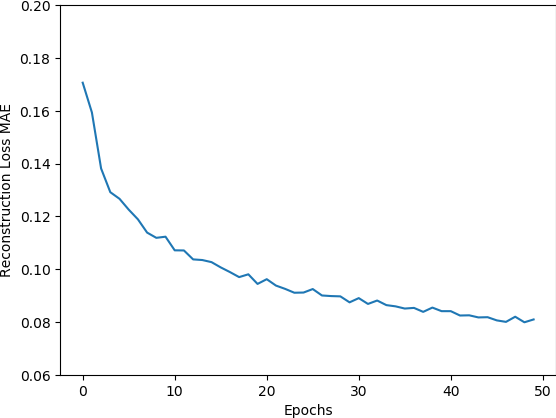
\includegraphics[width=\textwidth]
        {images/figures/experiments_architecture/mae_graphKernel3adjusted2x2x256_dim1024.png}
    \end{subfigure}%
    \begin{subfigure}{.5\textwidth}
      \begin{itemize}
          \item MAEs last epoch: $0.08655346$
          \item Mean loss last epoch: $0.08093627$
          \item Total weights: $3,935,651$
          \item Training time: $12$ min $58$ sec
      \end{itemize}
    \end{subfigure}
    \caption{The graph depicts the mean of all the mean average errors (MAEs)
    which were produced in the same epoch for every epoch. \textit{"MAEs last epoch"} is the mean of the MAEs
    of the batches in the last epoch, i.e. the last value of the graph. \textit{"Mean loss last epoch"} is the mean
    of the losses that the batches in the last epoch produced. Notice that this is not the same as the MAE since
    loss is the sum of the MAE and the Kullback-Leibler divergence. \textit{"Total weights"} is the number
    of weights in the network that are trained.}
\end{figure}

\begin{figure}[H]
    \centering
    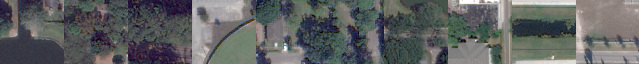
\includegraphics[width=\textwidth]
    {images/figures/experiments_architecture/inputsKernel3adjusted2x2x256_dim1024.png}
    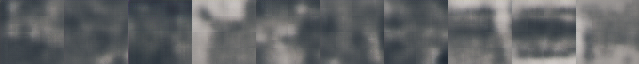
\includegraphics[width=\textwidth]
    {images/figures/experiments_architecture/reconstructionsKernel3adjusted2x2x256_dim1024.png}
    \caption{The original images in the top row are taken from a validation set
    that the VAE has not seen in training.
    The images in the bottom row are reconstructions of the original produced by the VAE after training.}
\end{figure}




\paragraph{Architecture 2}

\begin{center}
    \begin{table}[H]
        \centering
        \begin{tabular}{ | l | c | }
            \multicolumn{2}{c}{Encoder} \\ \hline
            Layer & Output\\ \hline
            Convolution: Kernel $3\times3$, Stride $2\times2$, Filters $16 $    & $64\times 64\times 16 $    \\  
            Convolution: Kernel $3\times3$, Stride $2\times2$, Filters $32 $    & $32\times 32\times 32 $    \\
            Convolution: Kernel $3\times3$, Stride $2\times2$, Filters $64 $    & $16\times 16\times 64 $    \\
            Convolution: Kernel $3\times3$, Stride $2\times2$, Filters $128$    & $8\times 8\times   128$    \\
            Convolution: Kernel $3\times3$, Stride $2\times2$, Filters $256$    & $4\times 4\times   256$    \\
            Convolution: Kernel $3\times3$, Stride $2\times2$, Filters $512$    & $2\times 2\times   512$    \\
            Flatten                                                             & $2,048$                    \\
            \hline
        \end{tabular} 
    \end{table}
\end{center}
\vspace{-4em}
\begin{center}
    \begin{table}[H]
        \centering
        \begin{tabular}{ | l | c | }
            \multicolumn{2}{c}{Decoder} \\ \hline
            Layer & Output\\ \hline
            Dense                                                                   & $2,048$                   \\
            Reshape                                                                 & $2\times 2\times    512$  \\
            Deconvolution: Kernel $3\times3$, Stride $2\times2$, Filters $256$      & $4\times 4\times    256$  \\  
            Deconvolution: Kernel $3\times3$, Stride $2\times2$, Filters $128$      & $8\times 8\times    128$  \\
            Deconvolution: Kernel $3\times3$, Stride $2\times2$, Filters $64 $      & $16\times 16\times  64 $  \\
            Deconvolution: Kernel $3\times3$, Stride $2\times2$, Filters $32 $      & $32\times 32\times  32 $  \\
            Deconvolution: Kernel $3\times3$, Stride $2\times2$, Filters $16 $      & $64\times 64\times  16 $  \\
            Deconvolution: Kernel $3\times3$, Stride $2\times2$, Filters $3  $      & $128\times 128\times3  $  \\
            \hline
        \end{tabular} 
    \end{table}
\end{center}

\vspace{-3em}

\begin{figure}[H]
    \centering
    \begin{subfigure}{.5\textwidth}
        \centering
        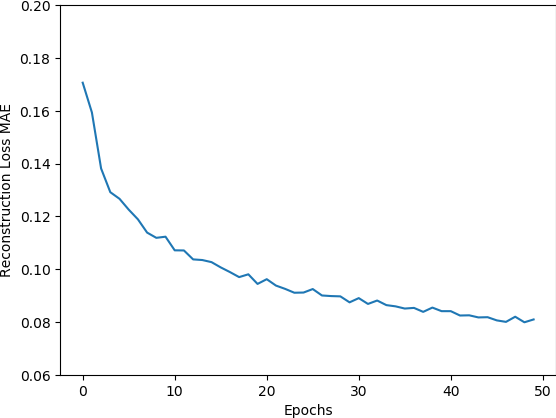
\includegraphics[width=\textwidth]
        {images/figures/experiments_architecture/mae_graphKernel3adjusted2x2x256_dim1024.png}
    \end{subfigure}%
    \begin{subfigure}{.5\textwidth}
      \begin{itemize}
          \item MAEs last epoch: $0.16682471$
          \item Mean loss last epoch: $0.16682471$
          \item Total weights: $9,440,579$
          \item Training time:
      \end{itemize}
    \end{subfigure}
\end{figure}

\vspace{-2em}

\begin{figure}[H]
    \centering
    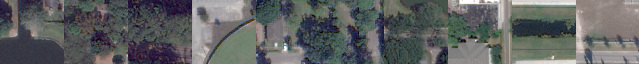
\includegraphics[width=\textwidth]
    {images/figures/experiments_architecture/inputsKernel3adjusted2x2x256_dim1024.png}
    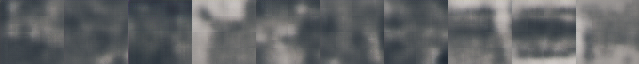
\includegraphics[width=\textwidth]
    {images/figures/experiments_architecture/reconstructionsKernel3adjusted2x2x256_dim1024.png}
\end{figure}

\paragraph{Architecture 3}

\begin{center}
    \begin{table}[H]
        \centering
        \begin{tabular}{ | l | c | }
            \multicolumn{2}{c}{Encoder} \\ \hline
            Layer & Output\\ \hline
            Convolution: Kernel $3\times3$, Stride $2\times2$, Filters $8  $    & $64\times 64\times 8  $    \\  
            Convolution: Kernel $3\times3$, Stride $2\times2$, Filters $16 $    & $32\times 32\times 16 $    \\
            Convolution: Kernel $3\times3$, Stride $2\times2$, Filters $32 $    & $16\times 16\times 32 $    \\
            Convolution: Kernel $3\times3$, Stride $2\times2$, Filters $64 $    & $8\times 8\times   64 $    \\
            Convolution: Kernel $3\times3$, Stride $2\times2$, Filters $128$    & $4\times 4\times   128$    \\
            Flatten                                                             & $2,048$                    \\
            \hline
        \end{tabular} 
    \end{table}
\end{center}
\vspace{-4em}
\begin{center}
    \begin{table}[H]
        \centering
        \begin{tabular}{ | l | c | }
            \multicolumn{2}{c}{Decoder} \\ \hline
            Layer & Output\\ \hline
            Dense                                                                   & $2,048$                   \\
            Reshape                                                                 & $4\times 4\times    128$  \\
            Deconvolution: Kernel $3\times3$, Stride $2\times2$, Filters $64 $      & $8\times 8\times    64 $  \\
            Deconvolution: Kernel $3\times3$, Stride $2\times2$, Filters $32 $      & $16\times 16\times  32 $  \\
            Deconvolution: Kernel $3\times3$, Stride $2\times2$, Filters $16 $      & $32\times 32\times  16 $  \\
            Deconvolution: Kernel $3\times3$, Stride $2\times2$, Filters $8  $      & $64\times 64\times  8  $  \\
            Deconvolution: Kernel $3\times3$, Stride $2\times2$, Filters $3  $      & $128\times 128\times3  $  \\
            \hline
        \end{tabular} 
    \end{table}
\end{center}

\vspace{-3em}

\begin{figure}[H]
    \centering
    \begin{subfigure}{.5\textwidth}
        \centering
        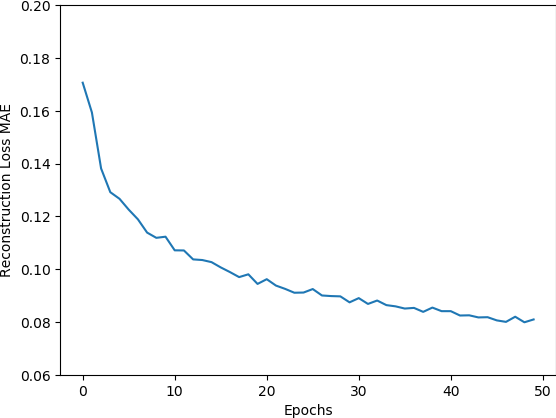
\includegraphics[width=\textwidth]
        {images/figures/experiments_architecture/mae_graphKernel3adjusted2x2x256_dim1024.png}
    \end{subfigure}%
    \begin{subfigure}{.5\textwidth}
      \begin{itemize}
          \item MAEs last epoch: $0.16682471$
          \item Mean loss last epoch: $0.16682471$
          \item Total weights: $6,492,192$
          \item Training time:
      \end{itemize}
    \end{subfigure}
\end{figure}

\vspace{-2em}

\begin{figure}[H]
    \centering
    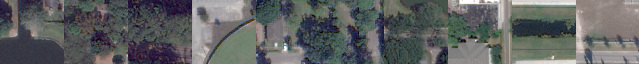
\includegraphics[width=\textwidth]
    {images/figures/experiments_architecture/inputsKernel3adjusted2x2x256_dim1024.png}
    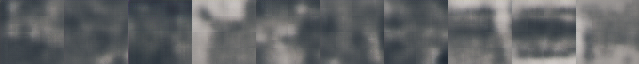
\includegraphics[width=\textwidth]
    {images/figures/experiments_architecture/reconstructionsKernel3adjusted2x2x256_dim1024.png}
\end{figure}

\paragraph{Architecture 4}

\begin{center}
    \begin{table}[H]
        \centering
        \begin{tabular}{ | l | c | }
            \multicolumn{2}{c}{Encoder} \\ \hline
            Layer & Output\\ \hline
            Convolution: Kernel $3\times3$, Stride $2\times2$, Filters $16 $    & $64\times 64\times 16 $    \\  
            Convolution: Kernel $3\times3$, Stride $2\times2$, Filters $32 $    & $32\times 32\times 32 $    \\
            Convolution: Kernel $3\times3$, Stride $2\times2$, Filters $64 $    & $16\times 16\times 64 $    \\
            Convolution: Kernel $3\times3$, Stride $2\times2$, Filters $128$    & $8\times 8\times   128$    \\
            Convolution: Kernel $3\times3$, Stride $2\times2$, Filters $256$    & $4\times 4\times   256$    \\
            Flatten                                                             & $4,096$                    \\
            \hline
        \end{tabular} 
    \end{table}
\end{center}
\vspace{-4em}
\begin{center}
    \begin{table}[H]
        \centering
        \begin{tabular}{ | l | c | }
            \multicolumn{2}{c}{Decoder} \\ \hline
            Layer & Output\\ \hline
            Dense                                                                   & $4,096$                   \\
            Reshape                                                                 & $4\times 4\times    256$  \\
            Deconvolution: Kernel $3\times3$, Stride $2\times2$, Filters $128$      & $8\times 8\times    128$  \\
            Deconvolution: Kernel $3\times3$, Stride $2\times2$, Filters $64 $      & $16\times 16\times  64 $  \\
            Deconvolution: Kernel $3\times3$, Stride $2\times2$, Filters $32 $      & $32\times 32\times  32 $  \\
            Deconvolution: Kernel $3\times3$, Stride $2\times2$, Filters $16 $      & $64\times 64\times  16 $  \\
            Deconvolution: Kernel $3\times3$, Stride $2\times2$, Filters $3  $      & $128\times 128\times3  $  \\
            \hline
        \end{tabular} 
    \end{table}
\end{center}

\vspace{-3em}

\begin{figure}[H]
    \centering
    \begin{subfigure}{.5\textwidth}
        \centering
        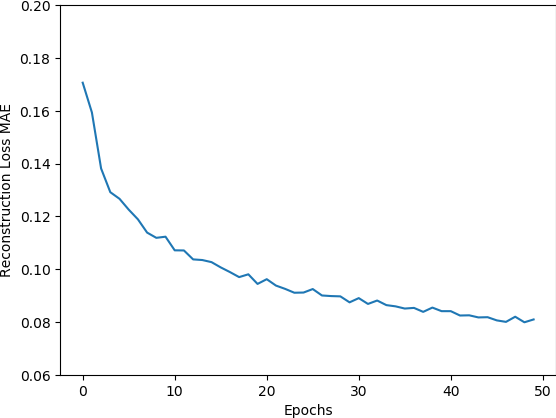
\includegraphics[width=\textwidth]
        {images/figures/experiments_architecture/mae_graphKernel3adjusted2x2x256_dim1024.png}
    \end{subfigure}%
    \begin{subfigure}{.5\textwidth}
      \begin{itemize}
          \item MAEs last epoch: $0.16682471$
          \item Mean loss last epoch: $0.16682471$
          \item Total weights: $13,374,019$
          \item Training time:
      \end{itemize}
    \end{subfigure}
\end{figure}

\vspace{-2em}

\begin{figure}[H]
    \centering
    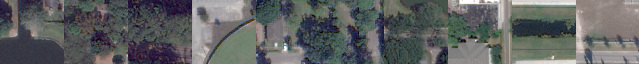
\includegraphics[width=\textwidth]
    {images/figures/experiments_architecture/inputsKernel3adjusted2x2x256_dim1024.png}
    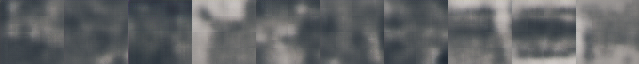
\includegraphics[width=\textwidth]
    {images/figures/experiments_architecture/reconstructionsKernel3adjusted2x2x256_dim1024.png}
\end{figure}

\paragraph{Architecture 5}

\begin{center}
    \begin{table}[H]
        \centering
        \begin{tabular}{ | l | c | }
            \multicolumn{2}{c}{Encoder} \\ \hline
            Layer & Output\\ \hline
            Convolution: Kernel $3\times3$, Stride $2\times2$, Filters $8  $    & $64\times 64\times 8  $    \\  
            Convolution: Kernel $3\times3$, Stride $2\times2$, Filters $16 $    & $32\times 32\times 16 $    \\
            Convolution: Kernel $3\times3$, Stride $2\times2$, Filters $32 $    & $16\times 16\times 32 $    \\
            Convolution: Kernel $3\times3$, Stride $2\times2$, Filters $64 $    & $8\times 8\times   64 $    \\
            Flatten                                                             & $4,096$                    \\
            \hline
        \end{tabular} 
    \end{table}
\end{center}
\vspace{-4em}
\begin{center}
    \begin{table}[H]
        \centering
        \begin{tabular}{ | l | c | }
            \multicolumn{2}{c}{Decoder} \\ \hline
            Layer & Output\\ \hline
            Dense                                                                   & $4,096$                   \\
            Reshape                                                                 & $8\times 8\times    64 $  \\
            Deconvolution: Kernel $3\times3$, Stride $2\times2$, Filters $32 $      & $16\times 16\times  32 $  \\
            Deconvolution: Kernel $3\times3$, Stride $2\times2$, Filters $16 $      & $32\times 32\times  16 $  \\
            Deconvolution: Kernel $3\times3$, Stride $2\times2$, Filters $8  $      & $64\times 64\times  8  $  \\
            Deconvolution: Kernel $3\times3$, Stride $2\times2$, Filters $3  $      & $128\times 128\times3  $  \\
            \hline
        \end{tabular} 
    \end{table}
\end{center}

\vspace{-3em}

\begin{figure}[H]
    \centering
    \begin{subfigure}{.5\textwidth}
        \centering
        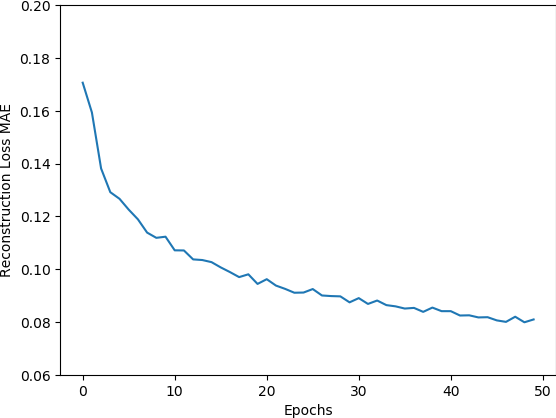
\includegraphics[width=\textwidth]
        {images/figures/experiments_architecture/mae_graphKernel3adjusted2x2x256_dim1024.png}
    \end{subfigure}%
    \begin{subfigure}{.5\textwidth}
      \begin{itemize}
          \item MAEs last epoch: $0.16682471$
          \item Mean loss last epoch: $0.16682471$
          \item Total weights: $12,638,051$
          \item Training time:
      \end{itemize}
    \end{subfigure}
\end{figure}

\vspace{-2em}

\begin{figure}[H]
    \centering
    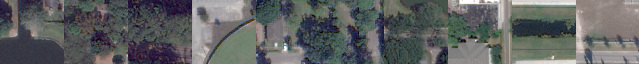
\includegraphics[width=\textwidth]
    {images/figures/experiments_architecture/inputsKernel3adjusted2x2x256_dim1024.png}
    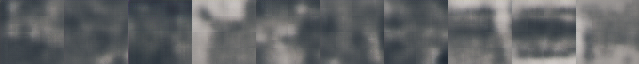
\includegraphics[width=\textwidth]
    {images/figures/experiments_architecture/reconstructionsKernel3adjusted2x2x256_dim1024.png}
\end{figure}



\paragraph{Architecture 6}

\begin{center}
    \begin{table}[H]
        \centering
        \begin{tabular}{ | l | c | }
            \multicolumn{2}{c}{Encoder} \\ \hline
            Layer & Output\\ \hline
            Convolution: Kernel $3\times3$, Stride $2\times2$, Filters $16 $    & $64\times 64\times 16 $    \\  
            Convolution: Kernel $3\times3$, Stride $2\times2$, Filters $32 $    & $32\times 32\times 32 $    \\
            Convolution: Kernel $3\times3$, Stride $2\times2$, Filters $64 $    & $16\times 16\times 64 $    \\
            Convolution: Kernel $3\times3$, Stride $2\times2$, Filters $128$    & $8\times 8\times   128$    \\
            Flatten                                                             & $8,192$                    \\
            \hline
        \end{tabular} 
    \end{table}
\end{center}
\vspace{-4em}
\begin{center}
    \begin{table}[H]
        \centering
        \begin{tabular}{ | l | c | }
            \multicolumn{2}{c}{Decoder} \\ \hline
            Layer & Output\\ \hline
            Dense                                                                   & $8,192$                   \\
            Reshape                                                                 & $8\times 8\times    128$  \\ 
            Deconvolution: Kernel $3\times3$, Stride $2\times2$, Filters $64 $      & $16\times 16\times  64 $  \\
            Deconvolution: Kernel $3\times3$, Stride $2\times2$, Filters $32 $      & $32\times 32\times  32 $  \\
            Deconvolution: Kernel $3\times3$, Stride $2\times2$, Filters $16 $      & $64\times 64\times  16 $  \\
            Deconvolution: Kernel $3\times3$, Stride $2\times2$, Filters $3  $      & $128\times 128\times3  $  \\
            \hline
        \end{tabular} 
    \end{table}
\end{center}

\vspace{-3em}

\begin{figure}[H]
    \centering
    \begin{subfigure}{.5\textwidth}
        \centering
        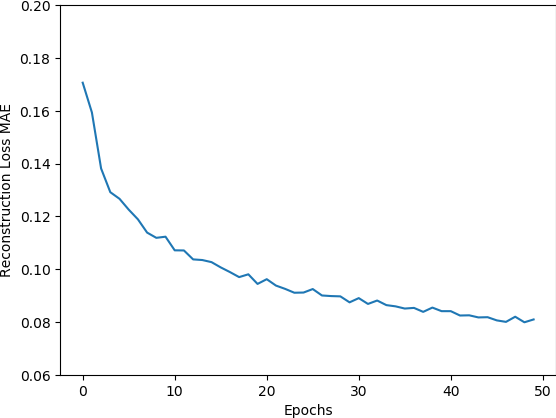
\includegraphics[width=\textwidth]
        {images/figures/experiments_architecture/mae_graphKernel3adjusted2x2x256_dim1024.png}
    \end{subfigure}%
    \begin{subfigure}{.5\textwidth}
      \begin{itemize}
          \item MAEs last epoch: $0.16682471$
          \item Mean loss last epoch: $0.16682471$
          \item Total weights: $25,376,819$
          \item Training time:
      \end{itemize}
    \end{subfigure}
\end{figure}

\vspace{-2em}

\begin{figure}[H]
    \centering
    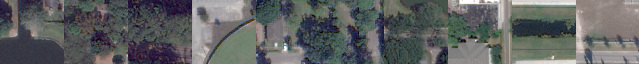
\includegraphics[width=\textwidth]
    {images/figures/experiments_architecture/inputsKernel3adjusted2x2x256_dim1024.png}
    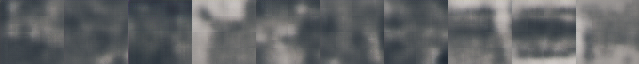
\includegraphics[width=\textwidth]
    {images/figures/experiments_architecture/reconstructionsKernel3adjusted2x2x256_dim1024.png}
\end{figure}



\paragraph{Architecture 7}

\begin{center}
    \begin{table}[H]
        \centering
        \begin{tabular}{ | l | c | }
            \multicolumn{2}{c}{Encoder} \\ \hline
            Layer & Output\\ \hline
            Convolution: Kernel $3\times3$, Stride $2\times2$, Filters $8  $    & $64\times 64\times 4  $    \\  
            Convolution: Kernel $3\times3$, Stride $2\times2$, Filters $16 $    & $32\times 32\times 8  $    \\
            Convolution: Kernel $3\times3$, Stride $2\times2$, Filters $32 $    & $16\times 16\times 16 $    \\
            Flatten                                                             & $4,096$                    \\
            \hline
        \end{tabular} 
    \end{table}
\end{center}
\vspace{-4em}
\begin{center}
    \begin{table}[H]
        \centering
        \begin{tabular}{ | l | c | }
            \multicolumn{2}{c}{Decoder} \\ \hline
            Layer & Output\\ \hline
            Dense                                                                   & $4,096$                   \\
            Reshape                                                                 & $16\times 16\times  16 $  \\
            Deconvolution: Kernel $3\times3$, Stride $2\times2$, Filters $8  $      & $32\times 32\times  8  $  \\
            Deconvolution: Kernel $3\times3$, Stride $2\times2$, Filters $4  $      & $64\times 64\times  4  $  \\
            Deconvolution: Kernel $3\times3$, Stride $2\times2$, Filters $3  $      & $128\times 128\times3  $  \\
            \hline
        \end{tabular} 
    \end{table}
\end{center}

\vspace{-3em}

\begin{figure}[H]
    \centering
    \begin{subfigure}{.5\textwidth}
        \centering
        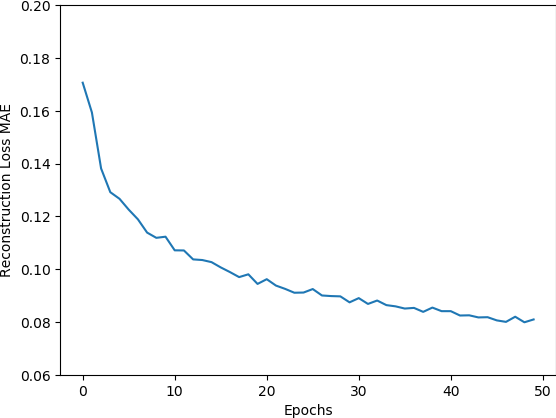
\includegraphics[width=\textwidth]
        {images/figures/experiments_architecture/mae_graphKernel3adjusted2x2x256_dim1024.png}
    \end{subfigure}%
    \begin{subfigure}{.5\textwidth}
      \begin{itemize}
          \item MAEs last epoch: $0.16682471$
          \item Mean loss last epoch: $0.16682471$
          \item Training time:
      \end{itemize}
    \end{subfigure}
\end{figure}

\vspace{-2em}

\begin{figure}[H]
    \centering
    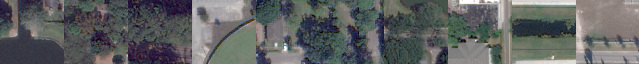
\includegraphics[width=\textwidth]
    {images/figures/experiments_architecture/inputsKernel3adjusted2x2x256_dim1024.png}
    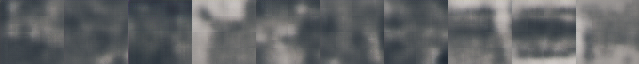
\includegraphics[width=\textwidth]
    {images/figures/experiments_architecture/reconstructionsKernel3adjusted2x2x256_dim1024.png}
\end{figure}



\paragraph{Architecture 8}

\begin{center}
    \begin{table}[H]
        \centering
        \begin{tabular}{ | l | c | }
            \multicolumn{2}{c}{Encoder} \\ \hline
            Layer & Output\\ \hline
            Convolution: Kernel $3\times3$, Stride $2\times2$, Filters $8  $    & $64\times 64\times 8  $    \\  
            Convolution: Kernel $3\times3$, Stride $2\times2$, Filters $16 $    & $32\times 32\times 16 $    \\
            Convolution: Kernel $3\times3$, Stride $2\times2$, Filters $32 $    & $16\times 16\times 32 $    \\
            Flatten                                                             & $8,192$                    \\
            \hline
        \end{tabular}
    \end{table}
\end{center}
\vspace{-4em}
\begin{center}
    \begin{table}[H]
        \centering
        \begin{tabular}{ | l | c | }
            \multicolumn{2}{c}{Decoder} \\ \hline
            Layer & Output\\ \hline
            Dense                                                                   & $8,192$                   \\
            Reshape                                                                 & $16\times 16\times  32 $  \\
            Deconvolution: Kernel $3\times3$, Stride $2\times2$, Filters $16 $      & $32\times 32\times  16 $  \\
            Deconvolution: Kernel $3\times3$, Stride $2\times2$, Filters $8  $      & $64\times 64\times  8  $  \\
            Deconvolution: Kernel $3\times3$, Stride $2\times2$, Filters $3  $      & $128\times 128\times3  $  \\
            \hline
        \end{tabular} 
    \end{table}
\end{center}

\vspace{-3em}

\begin{figure}[H]
    \centering
    \begin{subfigure}{.5\textwidth}
        \centering
        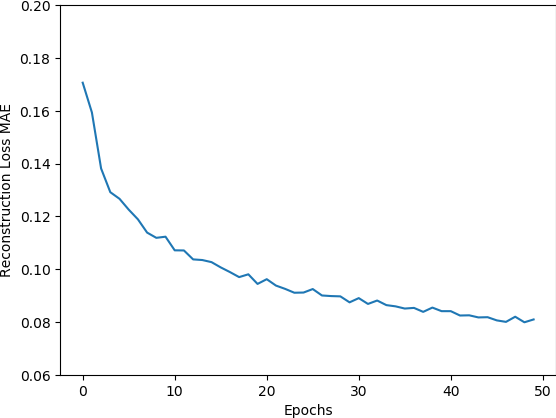
\includegraphics[width=\textwidth]
        {images/figures/experiments_architecture/mae_graphKernel3adjusted2x2x256_dim1024.png}
    \end{subfigure}%
    \begin{subfigure}{.5\textwidth}
      \begin{itemize}
          \item MAEs last epoch: $0.16682471$
          \item Mean loss last epoch: $0.16682471$
          \item Total weights: $25,188,099$
          \item Training time:
      \end{itemize}
    \end{subfigure}
\end{figure}

\vspace{-2em}

\begin{figure}[H]
    \centering
    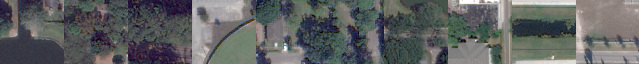
\includegraphics[width=\textwidth]
    {images/figures/experiments_architecture/inputsKernel3adjusted2x2x256_dim1024.png}
    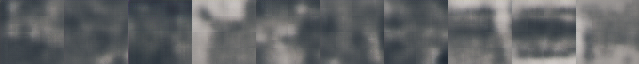
\includegraphics[width=\textwidth]
    {images/figures/experiments_architecture/reconstructionsKernel3adjusted2x2x256_dim1024.png}
\end{figure}



\paragraph{Architecture 9}

\begin{center}
    \begin{table}[H]
        \centering
        \begin{tabular}{ | l | c | }
            \multicolumn{2}{c}{Encoder} \\ \hline
            Layer & Output\\ \hline
            Convolution: Kernel $3\times3$, Stride $2\times2$, Filters $8  $    & $64\times 64\times 8  $    \\  
            Convolution: Kernel $3\times3$, Stride $2\times2$, Filters $16 $    & $32\times 32\times 16 $    \\
            Convolution: Kernel $3\times3$, Stride $1\times1$, Filters $16 $    & $32\times 32\times 16 $    \\
            Convolution: Kernel $3\times3$, Stride $1\times1$, Filters $16 $    & $32\times 32\times 16 $    \\
            Convolution: Kernel $3\times3$, Stride $1\times1$, Filters $16 $    & $32\times 32\times 16 $    \\
            Convolution: Kernel $3\times3$, Stride $2\times2$, Filters $32 $    & $16\times 16\times 32 $    \\
            Flatten                                                             & $8,192$                    \\
            \hline
        \end{tabular}
    \end{table}
\end{center}
\vspace{-4em}
\begin{center}
    \begin{table}[H]
        \centering
        \begin{tabular}{ | l | c | }
            \multicolumn{2}{c}{Decoder} \\ \hline
            Layer & Output\\ \hline
            Dense                                                                   & $8,192$                   \\
            Reshape                                                                 & $16\times 16\times  32 $  \\
            Deconvolution: Kernel $3\times3$, Stride $2\times2$, Filters $16 $      & $32\times 32\times  16 $  \\
            Deconvolution: Kernel $3\times3$, Stride $1\times1$, Filters $16 $      & $32\times 32\times  16 $  \\
            Deconvolution: Kernel $3\times3$, Stride $1\times1$, Filters $16 $      & $32\times 32\times  16 $  \\
            Deconvolution: Kernel $3\times3$, Stride $1\times1$, Filters $16 $      & $32\times 32\times  16 $  \\
            Deconvolution: Kernel $3\times3$, Stride $2\times2$, Filters $8  $      & $64\times 64\times  8  $  \\
            Deconvolution: Kernel $3\times3$, Stride $2\times2$, Filters $3  $      & $128\times 128\times3  $  \\
            \hline
        \end{tabular} 
    \end{table}
\end{center}

\vspace{-3em}

\begin{figure}[H]
    \centering
    \begin{subfigure}{.5\textwidth}
        \centering
        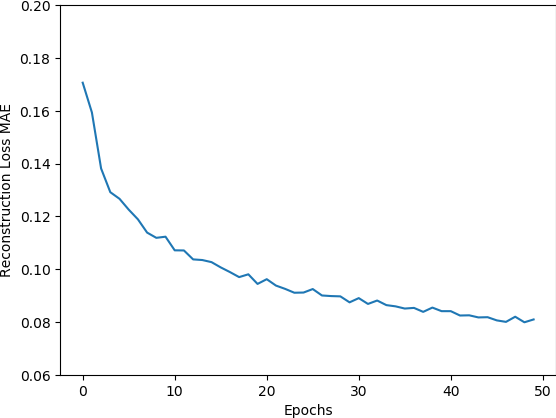
\includegraphics[width=\textwidth]
        {images/figures/experiments_architecture/mae_graphKernel3adjusted2x2x256_dim1024.png}
    \end{subfigure}%
    \begin{subfigure}{.5\textwidth}
      \begin{itemize}
          \item MAEs last epoch: $0.16682471$
          \item Mean loss last epoch: $0.16682471$
          \item Training time:
      \end{itemize}
    \end{subfigure}
\end{figure}

\vspace{-2em}

\begin{figure}[H]
    \centering
    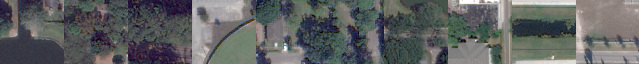
\includegraphics[width=\textwidth]
    {images/figures/experiments_architecture/inputsKernel3adjusted2x2x256_dim1024.png}
    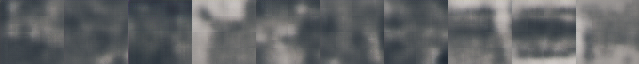
\includegraphics[width=\textwidth]
    {images/figures/experiments_architecture/reconstructionsKernel3adjusted2x2x256_dim1024.png}
\end{figure}



\paragraph{Architecture 10}

\begin{center}
    \begin{table}[H]
        \centering
        \begin{tabular}{ | l | c | }
            \multicolumn{2}{c}{Encoder} \\ \hline
            Layer & Output\\ \hline
            Convolution: Kernel $3\times3$, Stride $2\times2$, Filters $16 $    & $64\times 64\times 16 $    \\  
            Convolution: Kernel $3\times3$, Stride $2\times2$, Filters $32 $    & $32\times 32\times 32 $    \\
            Convolution: Kernel $3\times3$, Stride $2\times2$, Filters $64 $    & $16\times 16\times 64 $    \\
            Flatten                                                             & $16,384$                    \\
            \hline
        \end{tabular}
    \end{table}
\end{center}
\vspace{-4em}
\begin{center}
    \begin{table}[H]
        \centering
        \begin{tabular}{ | l | c | }
            \multicolumn{2}{c}{Decoder} \\ \hline
            Layer & Output\\ \hline
            Dense                                                                   & $16,384$                   \\
            Reshape                                                                 & $16\times 16\times  64 $  \\ 
            Deconvolution: Kernel $3\times3$, Stride $2\times2$, Filters $32 $      & $32\times 32\times  32 $  \\
            Deconvolution: Kernel $3\times3$, Stride $2\times2$, Filters $16 $      & $64\times 64\times  16 $  \\
            Deconvolution: Kernel $3\times3$, Stride $2\times2$, Filters $3  $      & $128\times 128\times3  $  \\
            \hline
        \end{tabular} 
    \end{table}
\end{center}

\vspace{-3em}

\begin{figure}[H]
    \centering
    \begin{subfigure}{.5\textwidth}
        \centering
        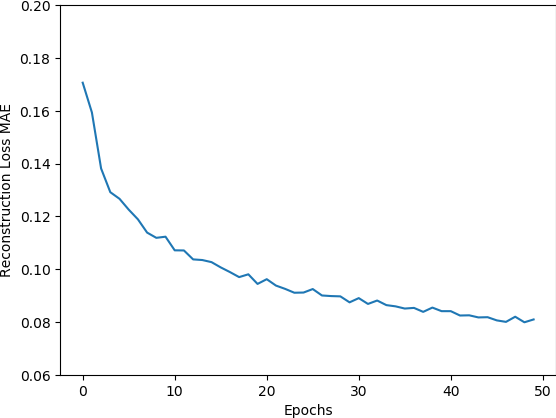
\includegraphics[width=\textwidth]
        {images/figures/experiments_architecture/mae_graphKernel3adjusted2x2x256_dim1024.png}
    \end{subfigure}%
    \begin{subfigure}{.5\textwidth}
      \begin{itemize}
          \item MAEs last epoch: $0.16682471$
          \item Mean loss last epoch: $0.16682471$
          \item Total weights: $50,397,187$
          \item Training time:
      \end{itemize}
    \end{subfigure}
\end{figure}

\vspace{-2em}

\begin{figure}[H]
    \centering
    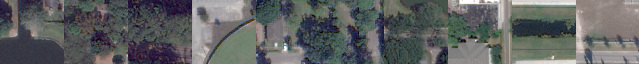
\includegraphics[width=\textwidth]
    {images/figures/experiments_architecture/inputsKernel3adjusted2x2x256_dim1024.png}
    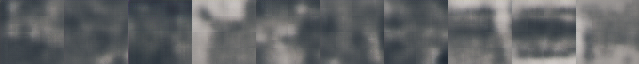
\includegraphics[width=\textwidth]
    {images/figures/experiments_architecture/reconstructionsKernel3adjusted2x2x256_dim1024.png}
\end{figure}




\paragraph{Architecture 11}

\begin{center}
    \begin{table}[H]
        \centering
        \begin{tabular}{ | l | c | }
            \multicolumn{2}{c}{Encoder} \\ \hline
            Layer & Output\\ \hline
            Convolution: Kernel $3\times3$, Stride $2\times2$, Filters $16 $    & $64\times 64\times 16 $    \\  
            Convolution: Kernel $3\times3$, Stride $2\times2$, Filters $32 $    & $32\times 32\times 32 $    \\
            Flatten                                                             & $32,768$                   \\
            \hline
        \end{tabular} 
    \end{table}
\end{center}
\vspace{-4em}
\begin{center}
    \begin{table}[H]
        \centering
        \begin{tabular}{ | l | c | }
            \multicolumn{2}{c}{Decoder} \\ \hline
            Layer & Output\\ \hline
            Dense                                                                   & $32,768$                  \\
            Reshape                                                                 & $32\times 32\times  32 $  \\ 
            Deconvolution: Kernel $3\times3$, Stride $2\times2$, Filters $16 $      & $64\times 64\times  16 $  \\
            Deconvolution: Kernel $3\times3$, Stride $2\times2$, Filters $3  $      & $128\times 128\times3  $  \\
            \hline
        \end{tabular} 
    \end{table}
\end{center}

\vspace{-3em}

\begin{figure}[H]
    \centering
    \begin{subfigure}{.5\textwidth}
        \centering
        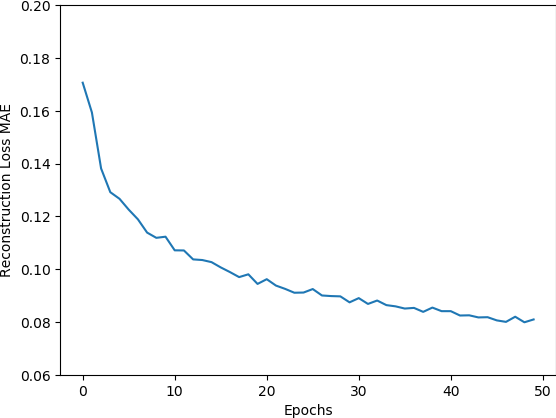
\includegraphics[width=\textwidth]
        {images/figures/experiments_architecture/mae_graphKernel3adjusted2x2x256_dim1024.png}
    \end{subfigure}%
    \begin{subfigure}{.5\textwidth}
      \begin{itemize}
          \item MAEs last epoch: $0.16682471$
          \item Mean loss last epoch: $0.16682471$
          \item Training time:
      \end{itemize}
    \end{subfigure}
\end{figure}

\vspace{-2em}

\begin{figure}[H]
    \centering
    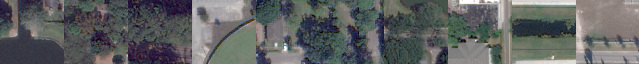
\includegraphics[width=\textwidth]
    {images/figures/experiments_architecture/inputsKernel3adjusted2x2x256_dim1024.png}
    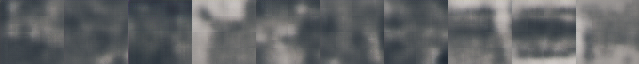
\includegraphics[width=\textwidth]
    {images/figures/experiments_architecture/reconstructionsKernel3adjusted2x2x256_dim1024.png}
\end{figure}

\paragraph{Architecture 12}

\begin{center}
    \begin{table}[H]
        \centering
        \begin{tabular}{ | l | c | }
            \multicolumn{2}{c}{Encoder} \\ \hline
            Layer & Output\\ \hline
            Convolution: Kernel $3\times3$, Stride $1\times1$, Filters $8  $    & $128\times 128\times 8  $    \\
            Avg Pool: Pool size $2\times2$                                      & $64\times 64\times   8  $    \\  
            Convolution: Kernel $3\times3$, Stride $1\times1$, Filters $16 $    & $64\times 64\times   16 $    \\
            Avg Pool: Pool size $2\times2$                                      & $32\times 32\times   16 $    \\
            Convolution: Kernel $3\times3$, Stride $1\times1$, Filters $32 $    & $32\times 32\times   32 $    \\
            Avg Pool: Pool size $2\times2$                                      & $16\times 16\times   32 $    \\
            Flatten                                                             & $8,192$                      \\
            \hline
        \end{tabular} 
    \end{table}
\end{center}
\vspace{-4em}
\begin{center}
    \begin{table}[H]
        \centering
        \begin{tabular}{ | l | c | }
            \multicolumn{2}{c}{Decoder} \\ \hline
            Layer & Output\\ \hline
            Dense                                                                   & $8,192$                   \\
            Reshape                                                                 & $16\times 16\times  32 $  \\
            Deconvolution: Kernel $3\times3$, Stride $2\times2$, Filters $16 $      & $32\times 32\times  16 $  \\
            Deconvolution: Kernel $3\times3$, Stride $2\times2$, Filters $8  $      & $64\times 64\times  8  $  \\
            Deconvolution: Kernel $3\times3$, Stride $2\times2$, Filters $3  $      & $128\times 128\times3  $  \\
            \hline
        \end{tabular} 
    \end{table}
\end{center}

\vspace{-3em}

\begin{figure}[H]
    \centering
    \begin{subfigure}{.5\textwidth}
        \centering
        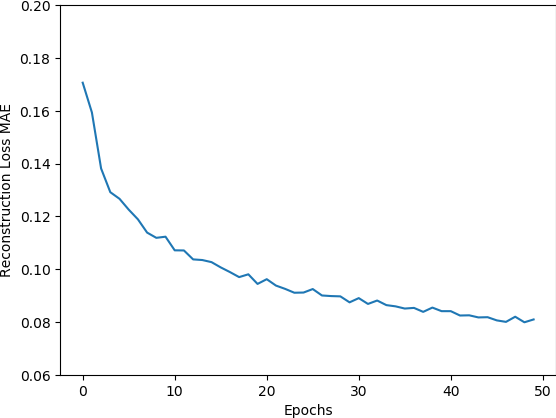
\includegraphics[width=\textwidth]
        {images/figures/experiments_architecture/mae_graphKernel3adjusted2x2x256_dim1024.png}
    \end{subfigure}%
    \begin{subfigure}{.5\textwidth}
      \begin{itemize}
          \item MAEs last epoch: $0.16682471$
          \item Mean loss last epoch: $0.16682471$
          \item Total weights: $25,376,819$
          \item Training time:
      \end{itemize}
    \end{subfigure}
\end{figure}

\vspace{-2em}

\begin{figure}[H]
    \centering
    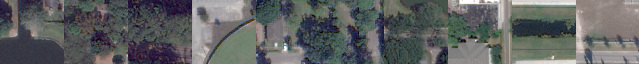
\includegraphics[width=\textwidth]
    {images/figures/experiments_architecture/inputsKernel3adjusted2x2x256_dim1024.png}
    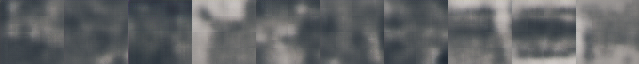
\includegraphics[width=\textwidth]
    {images/figures/experiments_architecture/reconstructionsKernel3adjusted2x2x256_dim1024.png}
\end{figure}



\paragraph{Architecture 13}

\begin{center}
    \begin{table}[H]
        \centering
        \begin{tabular}{ | l | c | }
            \multicolumn{2}{c}{Encoder} \\ \hline
            Layer & Output\\ \hline
            Convolution: Kernel $3\times3$, Stride $1\times1$, Filters $16 $    & $128\times 128\times 16  $    \\
            Avg Pooling: Pool size $2\times2$                                   & $64\times 64\times   16  $    \\  
            Convolution: Kernel $3\times3$, Stride $1\times1$, Filters $32 $    & $64\times 64\times   32 $    \\
            Avg Pooling: Pool size $2\times2$                                   & $32\times 32\times   32 $    \\
            Convolution: Kernel $3\times3$, Stride $1\times1$, Filters $64 $    & $32\times 32\times   64 $    \\
            Avg Pooling: Pool size $2\times2$                                   & $16\times 16\times   64 $    \\
            Flatten                                                             & $16,384$                      \\
            \hline
        \end{tabular} 
    \end{table}
\end{center}
\vspace{-4em}
\begin{center}
    \begin{table}[H]
        \centering
        \begin{tabular}{ | l | c | }
            \multicolumn{2}{c}{Decoder} \\ \hline
            Layer & Output\\ \hline
            Dense                                                                   & $16,384$                   \\
            Reshape                                                                 & $16\times 16\times  64 $  \\
            Deconvolution: Kernel $3\times3$, Stride $2\times2$, Filters $32 $      & $32\times 32\times  32 $  \\
            Deconvolution: Kernel $3\times3$, Stride $2\times2$, Filters $16 $      & $64\times 64\times  16 $  \\
            Deconvolution: Kernel $3\times3$, Stride $2\times2$, Filters $3  $      & $128\times 128\times3  $  \\
            \hline
        \end{tabular}
    \end{table}
\end{center}

\vspace{-3em}

\begin{figure}[H]
    \centering
    \begin{subfigure}{.5\textwidth}
        \centering
        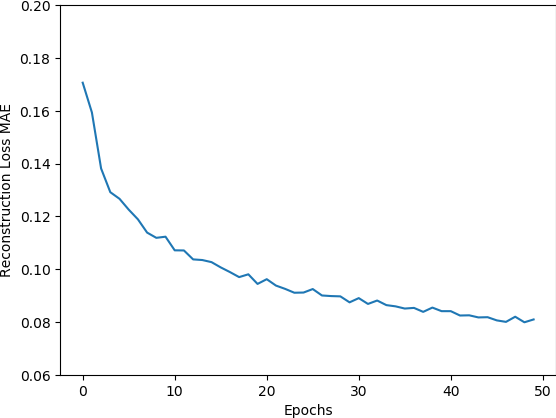
\includegraphics[width=\textwidth]
        {images/figures/experiments_architecture/mae_graphKernel3adjusted2x2x256_dim1024.png}
    \end{subfigure}%
    \begin{subfigure}{.5\textwidth}
      \begin{itemize}
          \item MAEs last epoch: $0.16682471$
          \item Mean loss last epoch: $0.16682471$
          \item Total weights: $50,397,187$
          \item Training time:
      \end{itemize}
    \end{subfigure}
\end{figure}

\vspace{-2em}

\begin{figure}[H]
    \centering
    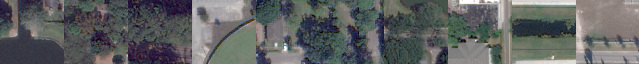
\includegraphics[width=\textwidth]
    {images/figures/experiments_architecture/inputsKernel3adjusted2x2x256_dim1024.png}
    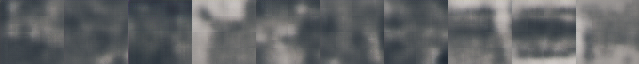
\includegraphics[width=\textwidth]
    {images/figures/experiments_architecture/reconstructionsKernel3adjusted2x2x256_dim1024.png}
\end{figure}




\paragraph{Architecture 14}

\begin{center}
    \begin{table}[H]
        \centering
        \begin{tabular}{ | l | c | }
            \multicolumn{2}{c}{Encoder} \\ \hline
            Layer & Output\\ \hline
            Convolution: Kernel $3\times3$, Stride $1\times1$, Filters $8  $    & $128\times 128\times 8  $    \\
            Max Pooling: Pool size $2\times2$                                   & $64\times 64\times   8  $    \\  
            Convolution: Kernel $3\times3$, Stride $1\times1$, Filters $16 $    & $64\times 64\times   16 $    \\
            Max Pooling: Pool size $2\times2$                                   & $32\times 32\times   16 $    \\
            Convolution: Kernel $3\times3$, Stride $1\times1$, Filters $32 $    & $32\times 32\times   32 $    \\
            Max Pooling: Pool size $2\times2$                                   & $16\times 16\times   32 $    \\
            Flatten                                                             & $8,192$                      \\
            \hline
        \end{tabular} 
    \end{table}
\end{center}
\vspace{-4em}
\begin{center}
    \begin{table}[H]
        \centering
        \begin{tabular}{ | l | c | }
            \multicolumn{2}{c}{Decoder} \\ \hline
            Layer & Output\\ \hline
            Dense                                                                   & $8,192$                   \\
            Reshape                                                                 & $16\times 16\times  32 $  \\
            Deconvolution: Kernel $3\times3$, Stride $2\times2$, Filters $16 $      & $32\times 32\times  16 $  \\
            Deconvolution: Kernel $3\times3$, Stride $2\times2$, Filters $8  $      & $64\times 64\times  8  $  \\
            Deconvolution: Kernel $3\times3$, Stride $2\times2$, Filters $3  $      & $128\times 128\times3  $  \\
            \hline
        \end{tabular} 
    \end{table}
\end{center}

\vspace{-3em}

\begin{figure}[H]
    \centering
    \begin{subfigure}{.5\textwidth}
        \centering
        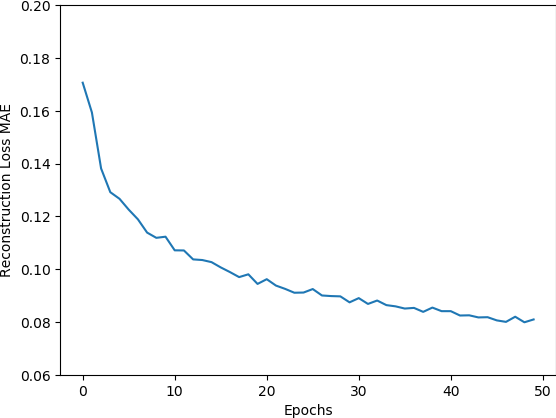
\includegraphics[width=\textwidth]
        {images/figures/experiments_architecture/mae_graphKernel3adjusted2x2x256_dim1024.png}
    \end{subfigure}%
    \begin{subfigure}{.5\textwidth}
      \begin{itemize}
          \item MAEs last epoch: $0.16682471$
          \item Mean loss last epoch: $0.16682471$
          \item Total weights: $25,376,819$
          \item Training time:
      \end{itemize}
    \end{subfigure}
\end{figure}

\vspace{-2em}

\begin{figure}[H]
    \centering
    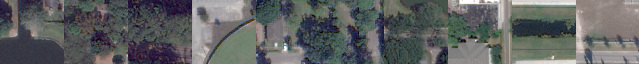
\includegraphics[width=\textwidth]
    {images/figures/experiments_architecture/inputsKernel3adjusted2x2x256_dim1024.png}
    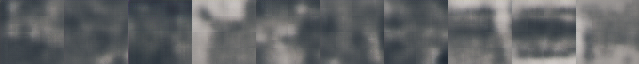
\includegraphics[width=\textwidth]
    {images/figures/experiments_architecture/reconstructionsKernel3adjusted2x2x256_dim1024.png}
\end{figure}




\paragraph{Architecture 15}

\begin{center}
    \begin{table}[H]
        \centering
        \begin{tabular}{ | l | c | }
            \multicolumn{2}{c}{Encoder} \\ \hline
            Layer & Output\\ \hline
            Convolution: Kernel $3\times3$, Stride $1\times1$, Filters $16 $    & $128\times 128\times 16  $    \\
            Max Pooling: Pool size $2\times2$                                   & $64\times 64\times   16  $    \\  
            Convolution: Kernel $3\times3$, Stride $1\times1$, Filters $32 $    & $64\times 64\times   32 $    \\
            Max Pooling: Pool size $2\times2$                                   & $32\times 32\times   32 $    \\
            Convolution: Kernel $3\times3$, Stride $1\times1$, Filters $64 $    & $32\times 32\times   64 $    \\
            Max Pooling: Pool size $2\times2$                                   & $16\times 16\times   64 $    \\
            Flatten                                                             & $16,384$                      \\
            \hline
        \end{tabular} 
    \end{table}
\end{center}
\vspace{-4em}
\begin{center}
    \begin{table}[H]
        \centering
        \begin{tabular}{ | l | c | }
            \multicolumn{2}{c}{Decoder} \\ \hline
            Layer & Output\\ \hline
            Dense                                                                   & $16,384$                   \\
            Reshape                                                                 & $16\times 16\times  64 $  \\
            Deconvolution: Kernel $3\times3$, Stride $2\times2$, Filters $32 $      & $32\times 32\times  32 $  \\
            Deconvolution: Kernel $3\times3$, Stride $2\times2$, Filters $16 $      & $64\times 64\times  16 $  \\
            Deconvolution: Kernel $3\times3$, Stride $2\times2$, Filters $3  $      & $128\times 128\times3  $  \\
            \hline
        \end{tabular}
    \end{table}
\end{center}

\vspace{-3em}

\begin{figure}[H]
    \centering
    \begin{subfigure}{.5\textwidth}
        \centering
        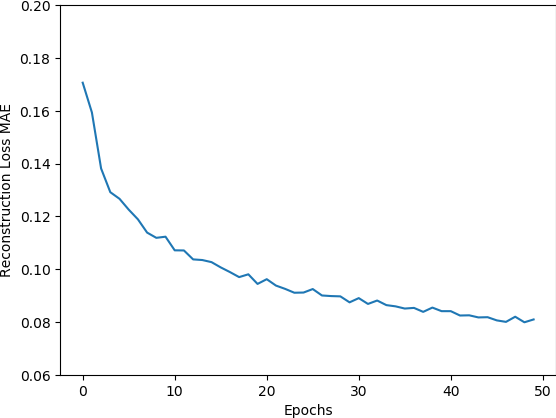
\includegraphics[width=\textwidth]
        {images/figures/experiments_architecture/mae_graphKernel3adjusted2x2x256_dim1024.png}
    \end{subfigure}%
    \begin{subfigure}{.5\textwidth}
      \begin{itemize}
          \item MAEs last epoch: $0.16682471$
          \item Mean loss last epoch: $0.16682471$
          \item Total weights: $50,397,187$
          \item Training time:
      \end{itemize}
    \end{subfigure}
\end{figure}

\vspace{-2em}

\begin{figure}[H]
    \centering
    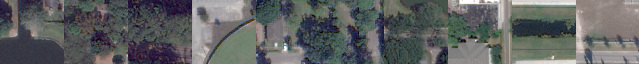
\includegraphics[width=\textwidth]
    {images/figures/experiments_architecture/inputsKernel3adjusted2x2x256_dim1024.png}
    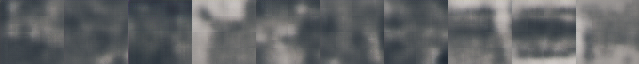
\includegraphics[width=\textwidth]
    {images/figures/experiments_architecture/reconstructionsKernel3adjusted2x2x256_dim1024.png}
\end{figure}

\paragraph{Architecture 16}

\begin{center}
    \begin{table}[H]
        \centering
        \begin{tabular}{ | l | c | }
            \multicolumn{2}{c}{Encoder} \\ \hline
            Layer & Output\\ \hline
            Convolution: Kernel $5\times5$, Stride $2\times2$, Filters $8  $    & $64\times 64\times 8  $    \\  
            Convolution: Kernel $5\times5$, Stride $2\times2$, Filters $16 $    & $32\times 32\times 16 $    \\
            Convolution: Kernel $5\times5$, Stride $2\times2$, Filters $32 $    & $16\times 16\times 32 $    \\
            Convolution: Kernel $5\times5$, Stride $2\times2$, Filters $64 $    & $8\times 8\times   64 $    \\
            Convolution: Kernel $5\times5$, Stride $2\times2$, Filters $128$    & $4\times 4\times   128$    \\
            Flatten                                                             & $2,048$                    \\
            \hline
        \end{tabular} 
    \end{table}
\end{center}
\vspace{-4em}
\begin{center}
    \begin{table}[H]
        \centering
        \begin{tabular}{ | l | c | }
            \multicolumn{2}{c}{Decoder} \\ \hline
            Layer & Output\\ \hline
            Dense                                                                   & $2,048$                   \\
            Reshape                                                                 & $4\times 4\times    128$  \\
            Deconvolution: Kernel $5\times5$, Stride $2\times2$, Filters $64 $      & $8\times 8\times    64 $  \\
            Deconvolution: Kernel $5\times5$, Stride $2\times2$, Filters $32 $      & $16\times 16\times  32 $  \\
            Deconvolution: Kernel $5\times5$, Stride $2\times2$, Filters $16 $      & $32\times 32\times  16 $  \\
            Deconvolution: Kernel $5\times5$, Stride $2\times2$, Filters $8  $      & $64\times 64\times  8  $  \\
            Deconvolution: Kernel $5\times5$, Stride $2\times2$, Filters $3  $      & $128\times 128\times3  $  \\
            \hline
        \end{tabular} 
    \end{table}
\end{center}

\vspace{-3em}

\begin{figure}[H]
    \centering
    \begin{subfigure}{.5\textwidth}
        \centering
        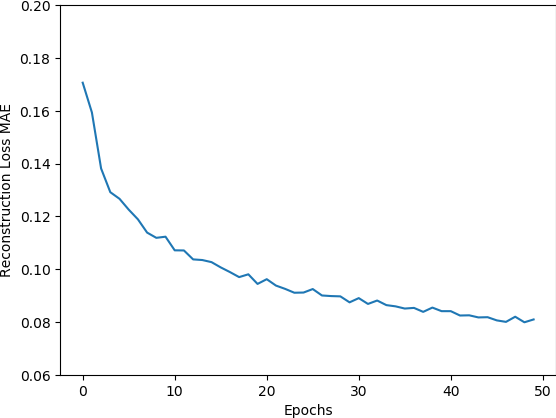
\includegraphics[width=\textwidth]
        {images/figures/experiments_architecture/mae_graphKernel3adjusted2x2x256_dim1024.png}
    \end{subfigure}%
    \begin{subfigure}{.5\textwidth}
      \begin{itemize}
          \item MAEs last epoch: $0.16682471$
          \item Mean loss last epoch: $0.16682471$
          \item Training time:
      \end{itemize}
    \end{subfigure}
\end{figure}

\vspace{-2em}

\begin{figure}[H]
    \centering
    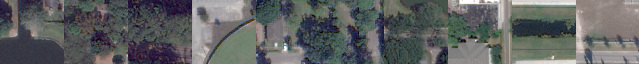
\includegraphics[width=\textwidth]
    {images/figures/experiments_architecture/inputsKernel3adjusted2x2x256_dim1024.png}
    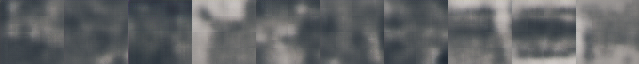
\includegraphics[width=\textwidth]
    {images/figures/experiments_architecture/reconstructionsKernel3adjusted2x2x256_dim1024.png}
\end{figure}

\paragraph{Architecture 17}

\begin{center}
    \begin{table}[H]
        \centering
        \begin{tabular}{ | l | c | }
            \multicolumn{2}{c}{Encoder} \\ \hline
            Layer & Output\\ \hline
            Convolution: Kernel $5\times5$, Stride $2\times2$, Filters $8  $    & $64\times 64\times 8  $    \\  
            Convolution: Kernel $5\times5$, Stride $2\times2$, Filters $16 $    & $32\times 32\times 16 $    \\
            Convolution: Kernel $5\times5$, Stride $2\times2$, Filters $32 $    & $16\times 16\times 32 $    \\
            Flatten                                                             & $8,192$                    \\
            \hline
        \end{tabular}
    \end{table}
\end{center}
\vspace{-4em}
\begin{center}
    \begin{table}[H]
        \centering
        \begin{tabular}{ | l | c | }
            \multicolumn{2}{c}{Decoder} \\ \hline
            Layer & Output\\ \hline
            Dense                                                                   & $8,192$                   \\
            Reshape                                                                 & $16\times 16\times  32 $  \\
            Deconvolution: Kernel $5\times5$, Stride $2\times2$, Filters $16 $      & $32\times 32\times  16 $  \\
            Deconvolution: Kernel $5\times5$, Stride $2\times2$, Filters $8  $      & $64\times 64\times  8  $  \\
            Deconvolution: Kernel $5\times5$, Stride $2\times2$, Filters $3  $      & $128\times 128\times3  $  \\
            \hline
        \end{tabular} 
    \end{table}
\end{center}

\vspace{-3em}

\begin{figure}[H]
    \centering
    \begin{subfigure}{.5\textwidth}
        \centering
        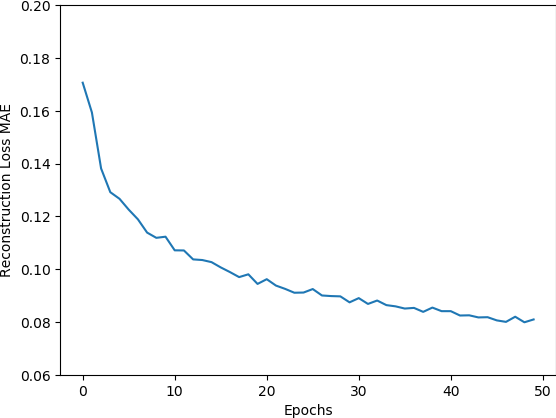
\includegraphics[width=\textwidth]
        {images/figures/experiments_architecture/mae_graphKernel3adjusted2x2x256_dim1024.png}
    \end{subfigure}%
    \begin{subfigure}{.5\textwidth}
      \begin{itemize}
          \item MAEs last epoch: $0.16682471$
          \item Mean loss last epoch: $0.16682471$
          \item Training time:
      \end{itemize}
    \end{subfigure}
\end{figure}

\vspace{-2em}

\begin{figure}[H]
    \centering
    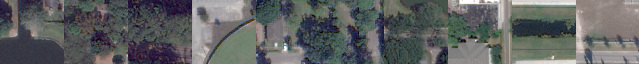
\includegraphics[width=\textwidth]
    {images/figures/experiments_architecture/inputsKernel3adjusted2x2x256_dim1024.png}
    \includegraphics[width=\textwidth]
    {images/figures/experiments_architecture/reconstructionsKernel3adjusted2x2x256_dim1024.png}
\end{figure}

\paragraph{Architecture 18}

\begin{center}
    \begin{table}[H]
        \centering
        \begin{tabular}{ | l | c | }
            \multicolumn{2}{c}{Encoder} \\ \hline
            Layer & Output\\ \hline
            Convolution: Kernel $3\times3$, Stride $1\times1$, Filters $8  $    & $128\times 128\times 8  $    \\
            Convolution: Kernel $3\times3$, Stride $2\times2$, Filters $8  $    & $64\times 64\times   8  $    \\
            Convolution: Kernel $3\times3$, Stride $1\times1$, Filters $16 $    & $64\times 64\times   16 $    \\
            Convolution: Kernel $3\times3$, Stride $2\times2$, Filters $16 $    & $32\times 32\times   16 $    \\
            Convolution: Kernel $3\times3$, Stride $1\times1$, Filters $32 $    & $32\times 32\times   32 $    \\
            Convolution: Kernel $3\times3$, Stride $2\times2$, Filters $32 $    & $16\times 16\times   32 $    \\
            Flatten                                                             & $8,192$                      \\
            \hline
        \end{tabular} 
    \end{table}
\end{center}
\vspace{-4em}
\begin{center}
    \begin{table}[H]
        \centering
        \begin{tabular}{ | l | c | }
            \multicolumn{2}{c}{Decoder} \\ \hline
            Layer & Output\\ \hline
            Dense                                                                   & $8,192$                   \\
            Reshape                                                                 & $16\times 16\times  32 $  \\
            Deconvolution: Kernel $3\times3$, Stride $2\times2$, Filters $16 $      & $32\times 32\times  16 $  \\
            Deconvolution: Kernel $3\times3$, Stride $2\times2$, Filters $8  $      & $64\times 64\times  8  $  \\
            Deconvolution: Kernel $3\times3$, Stride $2\times2$, Filters $3  $      & $128\times 128\times3  $  \\
            \hline
        \end{tabular} 
    \end{table}
\end{center}

\vspace{-3em}

\begin{figure}[H]
    \centering
    \begin{subfigure}{.5\textwidth}
        \centering
        \includegraphics[width=\textwidth]
        {images/figures/experiments_architecture/mae_graphKernel3adjusted2x2x256_dim1024.png}
    \end{subfigure}%
    \begin{subfigure}{.5\textwidth}
      \begin{itemize}
          \item MAEs last epoch: $0.16682471$
          \item Mean loss last epoch: $0.16682471$
          \item Training time:
      \end{itemize}
    \end{subfigure}
\end{figure}

\vspace{-2em}

\begin{figure}[H]
    \centering
    \includegraphics[width=\textwidth]
    {images/figures/experiments_architecture/inputsKernel3adjusted2x2x256_dim1024.png}
    \includegraphics[width=\textwidth]
    {images/figures/experiments_architecture/reconstructionsKernel3adjusted2x2x256_dim1024.png}
\end{figure}


\subsection{Latent Space} \label{latent_space_experiments}
